%!TEX root = ../main.tex

Sea $M$ una variedad topologica orientada y $Q\subset\text{Int}(M)$ finito.

\begin{definition}
    Un \textit{auto-homeomorfismo} de la pareja $(M,Q)$ es un homeomorfismo $f:M\to M$ tal que
    \begin{itemize}
        \item[i)] Para todo $x\in\partial M$,\, $f(x)=x$.
        \item[ii)] $f(Q)=Q.$ 
        \item[iii)] Preserva la orientacion.
    \end{itemize}
\end{definition}

Observe que en $i)$ cada punto de frontera esta fijo, mientras que por $ii)$ puede que $Q$ quede fijo pero tambien esta la posibilidad de permutar los puntos en $Q.$ 

Como es constumbre tenemos que definir una nocion de isotopia entre estos auto-homemomorfismos para poder empezar a dar la estructura adecuada y no estar repitiendo elementos.

\begin{definition}
    Sean $f_0,f_1$ auto-homeomorfismos de $(M,Q)$, decimos que son isotopicos si existe una familia de auto-homemomorfismos $\{f_t\}_{t\in I}$ donde estos sean los extremos y cada $f_t$ sea continuo.
\end{definition}
Dada la similitud con nociones anteriores no mostraremos que efectivamente esta isotopia define una relacion de equivalencia.
\begin{definition}
    El \textit{Mapping Class Group} $\mathcal{M}(M,Q)$ es el conjunto de clases de isotopia de automorfismos con la composicion de funciuones como operacion.
\end{definition}
Si el conjunto de puntos $Q=\varnothing$ omitiremos su escritura en general. A continuacion veremos un ejemplo clasico de este grupo
\begin{eg}
    Mostraremos que $\mathcal{M}(D^n)=\{1\},$ para esto consideremos la siguiente familia de funciones
    $$h_t(x)=\begin{cases}
        x&\text{si }t\leq|x|\leq 1,\\
        th\left(\dfrac{x}{t}\right)&\text{si }|x|<t.
    \end{cases}$$
   Donde $h$ es un auto-homemomorfismo de $D^n$. Note que $h_0=Id_{D^n}$, mientras que
   $$h_1=\begin{cases}
       x&\text{si }|x|=1,\\
       h(x)&\text{si }|x|<1.
   \end{cases}$$ 
   Que justamente es $h$ ya que este es auto-homeomorfismo. Claramente estos son continuos y son auto-homeomorfismos, asi concluimos lo deseado, en particular note que si $h(0)=0$, cada $h_t$ fija $0$ por lo que $\mathcal{M}(D^n,\{0\})=\{1\}.$
\end{eg}
En particular nos concentraremos en el caso $D^2$ y $Q\subset\int(M)$ un conjunto finito de puntos por lo anterior para un solo punto es el grupo trivial, de momento esto no resulta particularmente revelador pero al tomar $|Q|=k\geq 2$ se vera mejor la conexion pero no nos adelantemos.
\subsection{Medios-Giros}
Siguiendo las mismas nociones anteriores y con vistas en llegar a nociones de trenzas consideramos arcos especiales dentro de $D^2$
\begin{definition}
    Decimos que $\alpha$ es un \textit{arco generador} en $(M,Q)$ si
    \begin{itemize}
        \item $\alpha\subset M$ con $\alpha$ homeomorfico a $I.$
        \item $\alpha\cap(Q\cup\partial M)=\{x_1,x_2\}\subset Q$
    \end{itemize}
\end{definition}
Note que la primera condicion de ser homeomorfo evita que hallan autointersecciones en estos arcos, asi son lo que se suele llamar arcos simples. La segunda condicions hace referencia a que los arcos son disyuntos con $Q$ y la frontera de $M$ salvo en los extremos que son dos puntos exclusivamente de $Q$

\begin{eg}
Si tomamos $M=D^2$ y $Q=\left\{\pm\dfrac{1}{2}\right\}$, $\alpha$ es un arco generador donde sus extremos son los puntos de $Q.$
    \begin{center}
        

\tikzset{every picture/.style={line width=0.75pt}} %set default line width to 0.75pt        

\begin{tikzpicture}[x=0.75pt,y=0.75pt,yscale=-1.5,xscale=1.5]
%uncomment if require: \path (0,877); %set diagram left start at 0, and has height of 877

%Shape: Circle [id:dp9497408554436547] 
\draw   (190,145) .. controls (190,98.06) and (228.06,60) .. (275,60) .. controls (321.94,60) and (360,98.06) .. (360,145) .. controls (360,191.94) and (321.94,230) .. (275,230) .. controls (228.06,230) and (190,191.94) .. (190,145) -- cycle ;
%Straight Lines [id:da01695244465933632] 
\draw    (230,150) -- (320,150) ;

% Text Node
\draw (181,62.4) node [anchor=north west][inner sep=0.75pt]    {$D^{2}$};
% Text Node
\draw (267,122.4) node [anchor=north west][inner sep=0.75pt]    {$\alpha $};


\end{tikzpicture}
    \end{center}
\end{eg}

\begin{definition}
    Dado un arco generador $\alpha$ definimos el \textit{medio-giro} como
    $$\tau_\alpha\colon(M,Q)\to(M,Q)$$
    Tal que dada una vecindad pequeña $U$ de $\alpha$, que identificamos de manera homeomorfa con $\{z\in\C\colon|z|<1\}$ tal que $\alpha=\left[-\dfrac{1}{2},\dfrac{1}{2}\right]$ y la orientacion de $M$ sea en contra de las manecillas del reloj, tal que fuera de $U$, $\tau_\alpha$ es la identidad, Si $|z|\leq\dfrac{1}{2}$ es enviado a $-z$, y para $\dfrac{1}{2}\leq|z|<1$ es enviado a $ze^{-2\pi i|z|}$
\end{definition}
\begin{eg}
    Tomando como referencia el ejemplo anterior un Medio giro dado por $\tau_\alpha$ alteraria una curva transversal de la siguiente forma
    \begin{center}
        

\tikzset{every picture/.style={line width=0.75pt}} %set default line width to 0.75pt        

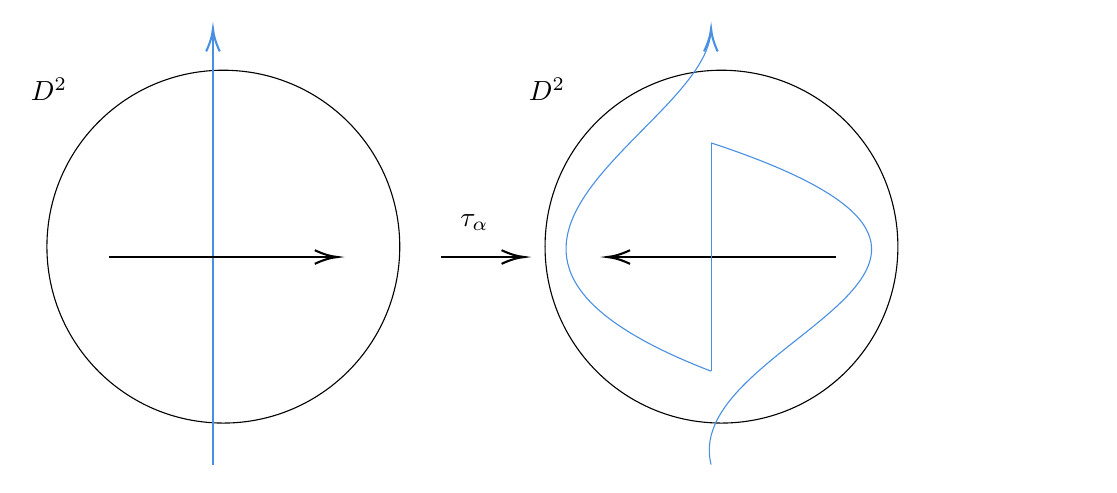
\begin{tikzpicture}[x=0.75pt,y=0.75pt,yscale=-1,xscale=1]
%uncomment if require: \path (0,877); %set diagram left start at 0, and has height of 877

%Shape: Circle [id:dp9497408554436547] 
\draw   (120,155) .. controls (120,108.06) and (158.06,70) .. (205,70) .. controls (251.94,70) and (290,108.06) .. (290,155) .. controls (290,201.94) and (251.94,240) .. (205,240) .. controls (158.06,240) and (120,201.94) .. (120,155) -- cycle ;
%Straight Lines [id:da6924922424889027] 
\draw [color={rgb, 255:red, 74; green, 144; blue, 226 }  ,draw opacity=1 ]   (200,260) -- (200,52) ;
\draw [shift={(200,50)}, rotate = 90] [color={rgb, 255:red, 74; green, 144; blue, 226 }  ,draw opacity=1 ][line width=0.75]    (10.93,-3.29) .. controls (6.95,-1.4) and (3.31,-0.3) .. (0,0) .. controls (3.31,0.3) and (6.95,1.4) .. (10.93,3.29)   ;
%Straight Lines [id:da4879924609046534] 
\draw    (150,160) -- (258,160) ;
\draw [shift={(260,160)}, rotate = 180] [color={rgb, 255:red, 0; green, 0; blue, 0 }  ][line width=0.75]    (10.93,-3.29) .. controls (6.95,-1.4) and (3.31,-0.3) .. (0,0) .. controls (3.31,0.3) and (6.95,1.4) .. (10.93,3.29)   ;
%Straight Lines [id:da7522321699548209] 
\draw    (310,160) -- (348,160) ;
\draw [shift={(350,160)}, rotate = 180] [color={rgb, 255:red, 0; green, 0; blue, 0 }  ][line width=0.75]    (10.93,-3.29) .. controls (6.95,-1.4) and (3.31,-0.3) .. (0,0) .. controls (3.31,0.3) and (6.95,1.4) .. (10.93,3.29)   ;
%Shape: Circle [id:dp5441253380968003] 
\draw   (360,155) .. controls (360,108.06) and (398.06,70) .. (445,70) .. controls (491.94,70) and (530,108.06) .. (530,155) .. controls (530,201.94) and (491.94,240) .. (445,240) .. controls (398.06,240) and (360,201.94) .. (360,155) -- cycle ;
%Straight Lines [id:da9790573072695838] 
\draw    (500,160) -- (392,160) ;
\draw [shift={(390,160)}, rotate = 360] [color={rgb, 255:red, 0; green, 0; blue, 0 }  ][line width=0.75]    (10.93,-3.29) .. controls (6.95,-1.4) and (3.31,-0.3) .. (0,0) .. controls (3.31,0.3) and (6.95,1.4) .. (10.93,3.29)   ;
%Straight Lines [id:da286317178551147] 
\draw [color={rgb, 255:red, 74; green, 144; blue, 226 }  ,draw opacity=1 ]   (440,105) -- (440,215) ;
%Curve Lines [id:da6408676567838075] 
\draw [color={rgb, 255:red, 74; green, 144; blue, 226 }  ,draw opacity=1 ]   (440,215) .. controls (284.57,155.1) and (436.4,99.62) .. (439.94,51.46) ;
\draw [shift={(440,50)}, rotate = 90.59] [color={rgb, 255:red, 74; green, 144; blue, 226 }  ,draw opacity=1 ][line width=0.75]    (10.93,-3.29) .. controls (6.95,-1.4) and (3.31,-0.3) .. (0,0) .. controls (3.31,0.3) and (6.95,1.4) .. (10.93,3.29)   ;
%Curve Lines [id:da7810815567546844] 
\draw [color={rgb, 255:red, 74; green, 144; blue, 226 }  ,draw opacity=1 ]   (440,105) .. controls (621.5,165) and (424.5,199) .. (440,260) ;

% Text Node
\draw (111,72.4) node [anchor=north west][inner sep=0.75pt]    {$D^{2}$};
% Text Node
\draw (318,138.4) node [anchor=north west][inner sep=0.75pt]    {$\tau _{\alpha }$};
% Text Node
\draw (351,72.4) node [anchor=north west][inner sep=0.75pt]    {$D^{2}$};


\end{tikzpicture}
    \end{center}
\end{eg}
Note que en terminos mas informales basicamente estamos rotando un $\alpha$ un angulo de $\pi$ fijando un punto medio, y todo lo demas se distorsiona acordemente. A continuacion enunciaremos mas no demostraremos las propiedades de estos medios giros
    \begin{itemize}
        \item Si $f\colon (M,Q)\to(M^\prime,Q^\prime)$ es un homeomorfismo que preserva la orientacion, y $\alpha$ un arco generador, entonces $f(\alpha)$ tambien lo es y $\tau_{f(\alpha)}=f\tau_\alpha f^{-1}.$
        \item Si $\alpha$ y $\alpha^\prime$ son isotopicos en la clase de arcos generadores, entonces $\tau_\alpha=\tau_{\alpha^\prime}$ en $\mathcal{M}(M,Q).$
        \item Si $\alpha,\beta$ son arcos generadores disjuntos en $\mathcal{M}(M,Q)$ entonces $\tau_\alpha\tau_\beta=\tau_\beta\tau_\alpha.$
        \item Para $\alpha,\beta$ arcos generadores que son disjuntos salvo un punto en comun en sus extremos tenemos que $\tau_\alpha\tau_\beta\tau_\alpha=\tau_\beta\tau_\alpha\tau_\beta.$
    \end{itemize}
    Observe la gran similitud inmediatamente con las relaciondes de trenzas, bastaria ver que tipo de arcos generadores son los que generarian el Mapping class group.

